\documentclass[a4paper, 12pt]{report}

\usepackage[margin=2cm]{geometry}
\usepackage{hyperref}

\usepackage{algorithm}
\usepackage{algpseudocode}

\usepackage{tikz}
\usetikzlibrary{shapes.geometric, arrows}

\usepackage{minted}

\title{Divide and Conquer Approach}
\author{Mouli Dutta}
\date{21-07-2023}


\setlength{\parindent}{0pt}
\renewcommand{\thesection}{\arabic{section}}


\tikzstyle{beginend} = [rectangle, rounded corners, minimum width=3cm, minimum height=1cm, text centered, draw=black, fill=blue!20]

\tikzstyle{process} = [rectangle, minimum width=3cm, minimum height=1cm, draw=black, fill=green!30, align=left]

\tikzstyle{decision} = [diamond, minimum width=3cm, minimum height=1cm, text centered, draw=black, aspect=2, fill=orange!30]

\tikzstyle{arrow} = [thick, ->, >=stealth]


\begin{document}
    \maketitle
    \tableofcontents
    \newpage
    
    \section{Introduction}

    The "Divide and Conquer" approach is a powerful algorithmic strategy used to solve complex problems by breaking them down into simpler sub-problems, solving each sub-problem independently, and then combining their solutions to obtain the final result. It is a fundamental algorithmic paradigm and is widely used in various fields, including computer science, mathematics, and engineering.\\
    
    The basic idea behind the divide and conquer approach is to divide a large problem into smaller, more manageable sub-problems, which are usually of the same type as the original problem but on a reduced input size. These sub-problems are solved recursively until they become simple enough to solve directly. Once the solutions to the sub-problems are obtained, they are combined to produce the solution to the original problem.\\

    The divide and conquer approach typically follows three main steps:\\

    \textbf{Divide}: The first step is to break down the original problem into smaller sub-problems. This division should be done in a way that each sub-problem resembles the original problem, but on a smaller scale. The goal is to simplify the problem and make it easier to handle.\\

    \textbf{Conquer}: Once the problem is divided into sub-problems, each sub-problem is solved independently. If the sub-problems are still complex, the algorithm will recursively apply the divide and conquer approach to further break them down into even smaller sub-problems until they become trivial enough to be solved directly.\\

    \textbf{Combine}: After obtaining the solutions to the sub-problems, the algorithm combines them to produce the final solution to the original problem.\\ \\

    
    \section {Example}

    A classic example of the divide and conquer approach is the "Merge Sort" algorithm, used to efficiently sort an array of elements. The algorithm divides the input array into two halves, recursively sorts each half, and then merges the two sorted halves to obtain the final sorted array.\\

    \newpage
    
    \section{Merge Sort Algorithm}
            
        \begin{algorithm}
        \caption{Algorithm for Merge}
            
            \begin{algorithmic}[1]
            
                \State \textbf{procedure:} Algorithm for Merge( Merge(A, low, high, mid))
                \State \textbf{Input:} Array A[low, high] is the input array and $mid = \frac{(low+high)}{2}$
                \State \textbf{Output:} Intermediate sorted array
                
                \State $i \gets low$
                \State $k \gets low$
                \State $j \gets mid + 1$
                
                \While {$(i \leq mid \ \&\& \ j \leq high)$}
                    \If{$(A[i] \leq A[j])$}
                        \State $B[k] \gets A[i]$ \Comment{B[low, high] is an auxiliary array}
                        \State $i \gets i + 1$
                    \Else
                        \State $B[k] \gets A[j]$
                        \State $j \gets j + 1$
                    \EndIf
                    \State $k \gets k + 1$
                \EndWhile
                
                \While{$(i \leq mid)$}
                    \State $B[k] \gets A[i]$
                    \State $i \gets i + 1$
                    \State $k \gets k + 1$
                \EndWhile
                
                \While{$(j \leq high)$}
                    \State $B[k] \gets A[j]$
                    \State $j \gets j + 1$
                    \State $k \gets k + 1$
                \EndWhile
    
                \For {$i \gets low$ to k in steps of 1}
                    \State $A[i] \gets B[i]$
                \EndFor
                    
            \end{algorithmic}
        \end{algorithm}

        \begin{algorithm}
        \caption{Algorithm for Merge Sort}
            \begin{algorithmic}[1]
                \State \textbf{procedure:} Algorithm for Merge Sort( MergeSort(A, low, high))
                \State \textbf{Input:} Array A[low, high] is the input array
                \State \textbf{Output:} The elements in non-decreasing order
                \If {$(low < high)$} \Comment{if runsize $!= 1$}
                    \State $mid \gets \frac{(low+high)}{2}$ \Comment{mid == midpoint}
                    \State \textit{MergeSort(A, low, mid)} \Comment{sort the left run}
                    \State \textit{MergeSort(A, mid+1, high)} \Comment{sort the right run}
                    \State \textit{Merge(A, low, high, mid)} \Comment{merge two intermediate sorted arrays A[low, mid] and A[mid+1, high]}
                \EndIf
                \State return
            \end{algorithmic}
        \end{algorithm}
            
    

    \newpage

    \section{Merge Sort Flowchart}
    
        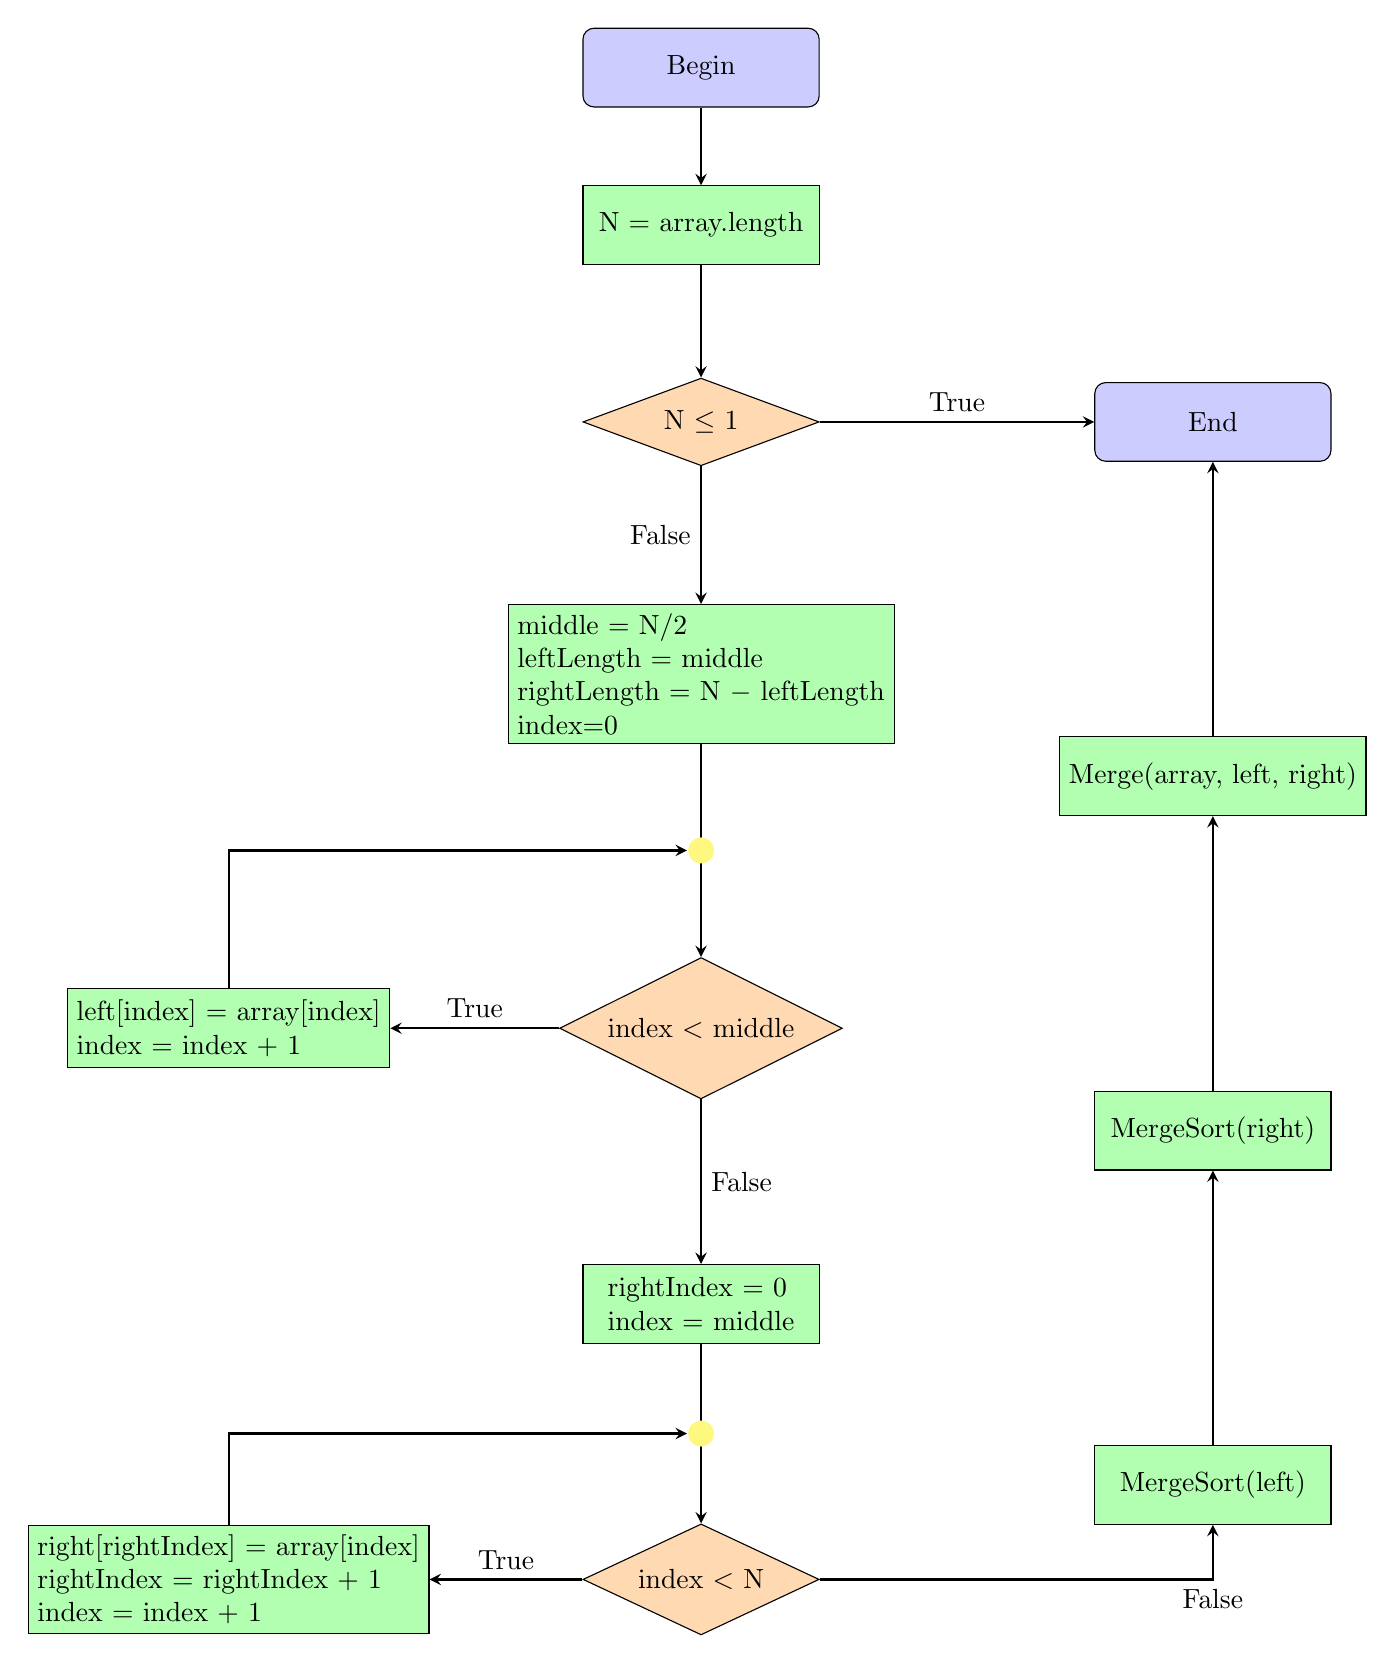
\begin{tikzpicture}[node distance = 2cm]
        
            \node (begin) [beginend] {Begin};
            
            \node (input) [process, below of=begin] {N = array.length};
            
            \node (base_cond) [decision, below of=input, yshift=-0.5cm] {N $\leq$ 1};
            
            \node (process1) [process, below of=base_cond, yshift=-1.2cm] {middle = N/2 \\ leftLength = middle \\ rightLength = N $-$ leftLength \\ index=0};
            
            \node(cond2) [decision, below of=process1, yshift=-2.5cm] {index $<$ middle};

            \node(process2) [process, left of=cond2, xshift=-4cm] {left[index] = array[index] \\index = index + 1};

            \node(process3) [process, below of=cond2, yshift=-1.5cm] {rightIndex = 0 \\ index = middle};

            \node(cond3) [decision, below of=process3, yshift=-1.5cm] {index $<$ N};

            \node(process5) [process, left of=cond3, xshift=-4cm] {right[rightIndex] = array[index] \\ rightIndex = rightIndex + 1 \\ index = index + 1};

            \node(end) [beginend, right of=base_cond, xshift=4.5cm] {End};

            \node(process8) [process, below of=end, yshift=-2.5cm] {Merge(array, left, right)};

            \node(process7) [process, below of=process8, yshift=-2.5cm] {MergeSort(right)};

            \node(process6) [process, below of=process7, yshift=-2.5cm] {MergeSort(left)};


            \draw [arrow] (begin) -- (input);
            \draw [arrow] (input) -- (base_cond);
            \draw [arrow] (base_cond) -- node[anchor=south] {True} (end);
            \draw [arrow] (base_cond) -- node[anchor=east] {False} (process1);
            \draw [arrow] (process1) -- node[fill=yellow!50, circle, midway](A){} (cond2);
            \draw [arrow] (process2) |- (A);
            \draw [arrow] (cond2.west) -- node[anchor=south] {True} (process2);
            \draw [arrow] (cond2) -- node[anchor=west] {False} (process3);
            \draw [arrow] (process3) -- node[fill=yellow!50, circle, midway](B){} (cond3);
            \draw [arrow] (process5) |- (B);
            \draw [arrow] (cond3.west) -- node[anchor=south]{True} (process5);
            \draw [arrow] (cond3.east) -| node[anchor=north] {False} (process6);
            \draw [arrow] (process6) -- (process7);
            \draw [arrow] (process7) -- (process8);
            \draw [arrow] (process8) -- (end);
            
            
        \end{tikzpicture}
        


    \newpage
    
    \section{Python code for Merge Sort}
        \begin{minted}{python}
        def merge_sort(arr):
            if len(arr) <= 1:
                return arr
        
            mid = len(arr) // 2
            left_half = merge_sort(arr[:mid])
            right_half = merge_sort(arr[mid:])
        
            return merge(left_half, right_half)
        
        def merge(left, right):
            merged_arr = []
            left_idx, right_idx = 0, 0
        
            while left_idx < len(left) and right_idx < len(right):
                if left[left_idx] < right[right_idx]:
                    merged_arr.append(left[left_idx])
                    left_idx += 1
                else:
                    merged_arr.append(right[right_idx])
                    right_idx += 1
        
            merged_arr.extend(left[left_idx:])
            merged_arr.extend(right[right_idx:])
        
            return merged_arr

        # Example usage:
        unsorted_list = [38, 27, 43, 3, 9, 82, 10]
        sorted_list = merge_sort(unsorted_list)
        print("Original List:", unsorted_list)
        print("Sorted List:", sorted_list)


        # Output:
        # Original List: [38, 27, 43, 3, 9, 82, 10]
        # Sorted List: [3, 9, 10, 27, 38, 43, 82]
        \end{minted}
    
\end{document}